\subsection*{\databaseName{}}\label{subsec:evaluation-db}
% SQL vs NoSQL
According to \citeauthor{flask_book2018}, \ac{sql} databases are a good choice for efficiently storing structured data.
This is because their paradigm \acs{acid}, i.e.\ \acl{acid}, provides high reliability.
\ac{nosql} databases, on the other hand, are more flexible and can be used to store unstructured data \cite{flask_book2018}.
They do not require a predefined schema and can therefore accept documents of arbitrary structure \cite{flask2018}.
Usually, \ac{nosql} databases do not offer services such as \texttt{JOIN}s.
%According to \citeauthor{flask2018}, \ac{nosql} databases make a tradeoff between storage and speed, as well as a tradeoff between consistency and availability.
\ac{nosql} databases are said to outperform out-of-the-box \ac{sql} databases.
Since the dataset consists of unstructured documents and the task at hand does not require performing any \texttt{JOIN}s, 
a \ac{nosql} database is favourable.
\databaseName{} is chosen since it is well known to provide near real-time search and to operate on big data.
Subsequently, it is a good fit for the underlying dataset.

% limited dimensionality elastic search
Since \databaseName{} stores vectors of at most 2048 dimensions,
the \ac{tfidf} and \infersent{} embeddings are problematic.
Besides imposing limits to the dimensionality of the embeddings, \databaseName{} offers a variety of convenient functionalities,
such as the built-in \ac{knn} search.
Therefore, in this work, \databaseName{} is used regardless of the dimensionality constraints imposed by the database.
Hence, the techniques are adjusted to the database and not vice versa.

% separation of initialisation and insertion
The time necessary to fill the \databaseName{} database has been evaluated and improved throughout this work.
The current time measurements are shown in \autoref{fig:time_init_db}.
The times correspond to calculation of 2048 embeddings.
It is possible to measure this compuation time individually since the task of filling the database is modulized. 
Modulizing is beneficial since it is possible to update the embeddings without having to recreate the database. 
Moreover, it facilitates debugging and comparing the models used to create the embeddings.

\begin{figure}[!htb] % htp = hier (h), top (t), oder auf einer eigenen Seite (p).
    \centering
    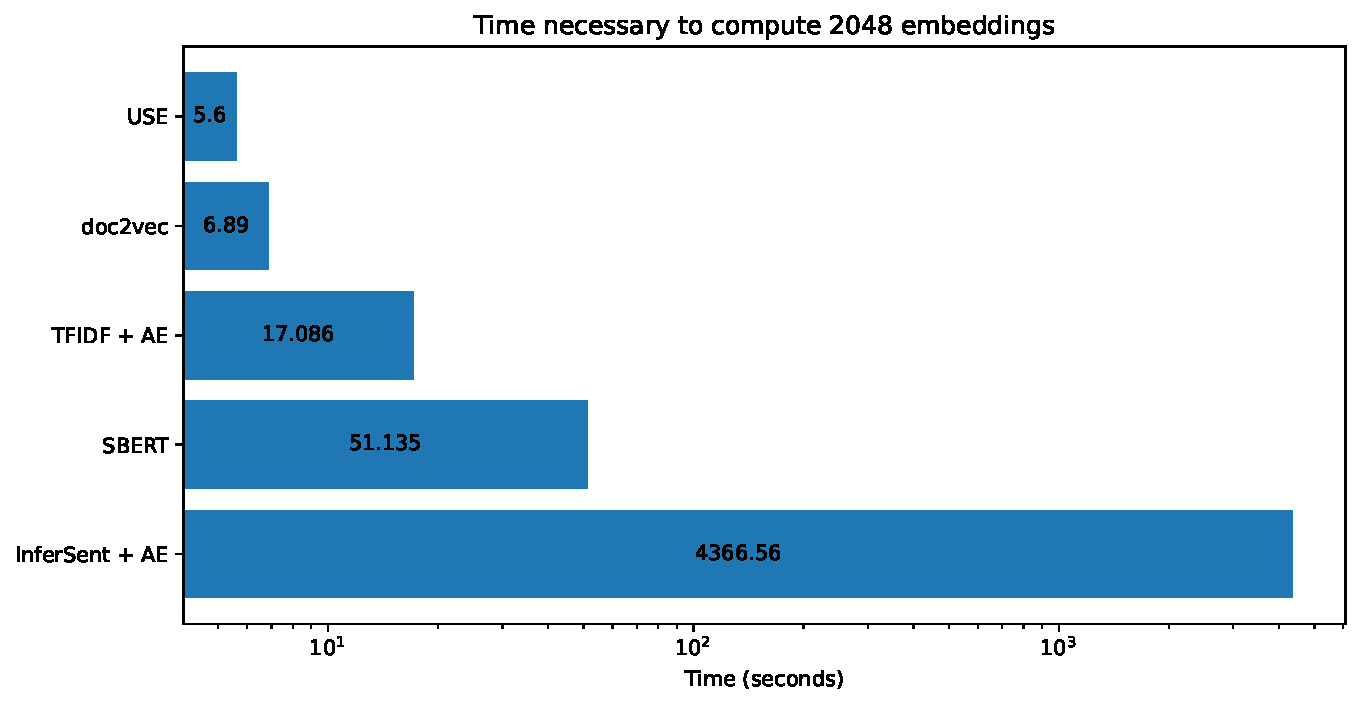
\includegraphics[width=1\textwidth]{images/Elasticsearch/Time_necessary_to_compute_2048_embeddings_log.pdf}
    \caption[Times for creating the database]{Time per module of creating the Bahamas database using a random selection of 2048 documents.
    The x-axis is logarithmic.
    The reference time is measured using \texttt{cProfiler} on a \localMaschineStats{}.
    %the \texttt{timer} from \texttt{timeit.default\_timer} on a \localMaschineStats{}.
    }
    \label{fig:time_init_db}
\end{figure}